\documentclass[12pt]{article}
\usepackage{color}
\usepackage[usenames,dvipsnames,svgnames,table]{xcolor}
\definecolor{dark-red}{rgb}{0.7,0.15,0.15} 
\usepackage[margin=1in]{geometry}
\usepackage[linkcolor=blue,
colorlinks=true,
urlcolor=blue,
pdfstartview={XYZ null null 1.00},
citecolor={blue},
pdftitle={In-N-Out}]{hyperref}
\usepackage[multiple]{footmisc}
\renewcommand{\footnotelayout}{\raggedright}
\usepackage{setspace} 
\usepackage{indentfirst}

\usepackage{verbatim}

\usepackage{Sweave}



\usepackage{titlesec}
\titleformat{\section}{\normalfont \centering}{\thesection}{.5em}{}
\titleformat{\subsection}{\normalfont}{\thesection}{.5em}{}
\setlength{\footnotesep}{0.5cm}

\let\proglang=\texttt
\newcommand{\pkg}[1]{{\fontseries{b}\selectfont #1}}

\newcommand{\superscript}[1]{\ensuremath{^{\textrm{#1}}}}

\usepackage{graphicx}

\usepackage{amsfonts,amssymb,amsbsy}
\usepackage{amsxtra}
\usepackage{amsmath}
\renewcommand{\thefootnote}{\fnsymbol{footnote}}

\usepackage{dcolumn}
\newcolumntype{.}{D{.}{.}{5}}
\newcolumntype{q}{D{.}{.}{3}}
	
\usepackage{natbib}
\bibpunct[, ]{(}{)}{;}{a}{}{,}

\usepackage{amsmath}

\raggedright
\parindent=1.5em % <- or whatever indent you want


\begin{document}
\doublespacing
\vspace{2cm}

\begin{center}
Explaining Partisan Affect\\Partisans Respond to Partisan Response\\ 
\vspace{2cm}
\today\\\vspace{2cm}

Doug Ahler\footnote{Doug Ahler is Ph.D. candidate in Political Science at the
University of California, Berkeley. Doug can be reached at
\href{mailto:dahler@berkeley.edu}{dahler@berkeley.edu}} and Gaurav
Sood\footnote{Gaurav Sood is a National Fellow at the Hoover Institution at
Stanford University. Gaurav can be reached at
\href{mailto:gsood@stanford.edu}{gsood@stanford.edu}}

\end{center}

\setcounter{page}{0}
\thispagestyle{empty}
\renewcommand*{\thefootnote}{\arabic{footnote}}
\newpage
\setcounter{footnote}{1}


\begin{comment}
	sweaver(paste0(basedir, "xperceive/partisanResponse/manuscript"), "presponse")
\end{comment}
\newpage

Partisans dislike supporters of the opposing party \citep{iyengar2012,
iyengar2013}. Sizable proportions of Democrats and Republicans say they would be
unhappy if a family member of theirs married someone from the opposing party
\citep{iyengar2012}. This widespread mutual antipathy exists despite a vast overlap in policy positions of supporters of both parties \citep{fiorina2012}. If policy differences don't explain this affective gulf, what does?

Ideologically extreme partisan elites draw considerable support from their own
party \citep{sood2013}. However, the support is not as well-founded in actual
agreement over policy as it is in \textit{perceived} agreement over policy. As
we later show, partisans also tend not to penalize elites of their own party for
their missteps. Whatever the reasons for tepid reactions to prominent missteps
by policitians of their own party, be it ignorance or partisan
selective exposure or greater faith in denials from one's own party
members, we show that information about these tepid reactions riles the
supporters of the opposing party.

We start by documenting partisans' tepid reactions to missteps by their own
party's elites. We document this using a new database of political scandals, coupled with opinion data from 2000 state level polls measuring approval of Senators, Governors, and the President. We supplement the public opinion data with national panel data from the National Annenberg Election Studies (NAES) and the National Election Studies. We use an interrupted time-series design to measure public opinion before and after political scandals. We find that partisans tend not to update evaluations of embattled leaders. Next, we experimentally manipulate the level of approval that leaders enjoy among their party's supporters following political debacles. We find that negative evaluations of outparty supporters increase when they continue to support embattled leaders, vis-a-vis when outparty supporters withdraw their support.

\section*{Partisans Respond to Partisan Response}
We randomly assign respondents to read about differing partisan responses to party elites' political errors. We thus create a counterfactual for identifying the effect of perceived outparty intransigence on affect toward the outparty.

\subsection*{Research Design}
In November 2013, we recruited 930 survey participants through Amazon's
Mechanical Turk \citep[see][]{BerinskyHuberLenz2012}. We randomly assigned participants to read a news story on one of three ongoing political scandals at the time: the troubled rollout of the U.S. health exchange website (Democratic Party blunder), Ted Cruz's inflammatory rhetoric precluding compromise during the shutdown and debt ceiling negotiations (Republican Party blunder), and Toronto mayor Rob Ford's drug scandal (control condition). Within news stories on American party leaders' political errors, we randomly assigned participants to one of two conditions related to partisan reaction. In one condition (``response''), participants read that support for the embattled elite (Obama or Cruz) declined among co-partisan citizens. In the other condition, (``no response''), participants read that support for the elite remained steadily high. See Appendix A for a complete transcript of the stories.

We assessed whether exposure to stories in which partisans withdraw support from
their party's elites when they learn about the political scandal, compared to
both, the control group, and the condition in which partisans continue to
support their leaders despite the political scandal, changed what partisans of
the opposing party believed of the supporters of the party whose elite was
embroiled in the scandal. In particular, after exposing respondents to the
stories, we asked the respondents how well they thought each of the following
eight traits -ignorant, sincere, open to reason, smug, selfish, patriotic,
compassionate, and hypocritical- described ``people who support the Democratic
(Republican) Party'' on a semantic five-point scale, ranging from ``extremely
well'' to ``not at all.'' We recoded ratings on negatively-valenced traits so
that all trait ratings ranged from negative to positive. We next created
a difference score as a summary measure of partisan affect (The $\alpha$ for
difference ratings was .90).

On the thinking that the effects would be moderated by respondent's level of
political interest, and political knowledge, we also measured these variables. 
Respondent's partisan identification was measured using the conventional
branched question found in the NES.

\section*{Analyses and Results}

As part of our survey and before random assignment to the conditions, we
measured whether or not the respondents were paying attention to the survey. In particular, we posed a question that asked respondents to mark two particular responses. Of the 930 respondents, 38 respondents failed to do the task as requested. We removed these participants from our sample as we felt that they were merely adding noise to the data.

Given our theory and the nature of the intervention, we further limit ourselves
to analyzing responses from partisans from the two major parties (both, those who lean towards any of the two parties, and those who identify themselves as partisans of any of the two parties). This limits our respondent pool to 726.

Within Mechanical Turk, there is typically a vast bias towards Democrats. More
than three-quarters of the 726 respondents -552- either leaned towards the
Democratic party or identified as Democrats outright. In the interests of
clarity but also in line with where most of our data lies, we first start by
analyzing data from Democrats. Furthermore, since our theory has to do with how
partisans react to how supporters of the opposing party react in reaction to
their elites' missteps, we analyze data from control, Republican's 'Change',
and republicans 'No Change' conditions.

Compared to control, R No Change causes increase in antipathy towards
Republicans (b = .06, $p < .11$, see Table 1). 

\centerline{Insert Table 1 here}

Effect is substantially greater
among Strong/Weak Democrats (taking out leaners), and among those with at least some basic levels of political
knowledge.


\clearpage
\singlespacing

\bibliographystyle{apsr_fs}
\bibliography{xperceive}  

\clearpage 
\section*{Tables}
\begin{table}[!ht]
\caption{Within Democrats}
\label{} 
\begin{tabular}{ l D{.}{.}{2}D{.}{.}{2}D{.}{.}{2} } 
\hline 
  & \multicolumn{ 1 }{ c }{ R-D Trt } & \multicolumn{ 1 }{ c }{ R-D Trt } & \multicolumn{ 1 }{ c }{ R-D Trt } \\ \hline
 %                & R-D Trt & R-D Trt & R-D Trt\\ 
(Intercept)      & 0.35 ^* & 0.35 ^* & 0.34 ^*\\ 
                 & (0.02)  & (0.03)  & (0.02) \\ 
treatD Change    & -0.06   &         &        \\ 
                 & (0.03)  &         &        \\ 
treatD No Change & -0.03   &         &        \\ 
                 & (0.03)  &         &        \\ 
treatR Change    & -0.01   & -0.01   &        \\ 
                 & (0.03)  & (0.03)  &        \\ 
treatR No Change & 0.06    & 0.06    & 0.07   \\ 
                 & (0.04)  & (0.04)  & (0.03)  \\
 $N$              & 552     & 319     & 219    \\ 
$R^2$            & 0.02    & 0.01    & 0.02   \\ 
adj. $R^2$       & 0.02    & 0.01    & 0.01   \\ 
Resid. sd        & 0.25    & 0.25    & 0.26    \\ \hline
 \multicolumn{4}{l}{\footnotesize{Standard errors in parentheses}}\\
\multicolumn{4}{l}{\footnotesize{$^*$ indicates significance at $p< 0.05 $}} 
\end{tabular} 
 \end{table}\begin{table}[!ht]
\caption{Within Democrats}
\label{} 
\begin{tabular}{ l D{.}{.}{2}D{.}{.}{2}D{.}{.}{2} } 
\hline 
  & \multicolumn{ 1 }{ c }{ Str./Weak Dems. } & \multicolumn{ 1 }{ c }{ Strong Dems. } & \multicolumn{ 1 }{ c }{ Know > 0 } \\ \hline
 %                & Str./Weak Dems. & Strong Dems.    & Know > 0       \\ 
(Intercept)      & 0.36 ^*         & 0.38 ^*         & 0.35 ^*        \\ 
                 & (0.03)          & (0.04)          & (0.04)         \\ 
treatR Change    & 0.01            & 0.07            & 0.02           \\ 
                 & (0.04)          & (0.05)          & (0.05)         \\ 
treatR No Change & 0.11 ^*         & 0.25 ^*         & 0.12 ^*        \\ 
                 & (0.04)          & (0.05)          & (0.05)          \\
 $N$              & 238             & 105             & 157            \\ 
$R^2$            & 0.03            & 0.18            & 0.04           \\ 
adj. $R^2$       & 0.03            & 0.16            & 0.03           \\ 
Resid. sd        & 0.26            & 0.23            & 0.25            \\ \hline
 \multicolumn{4}{l}{\footnotesize{Standard errors in parentheses}}\\
\multicolumn{4}{l}{\footnotesize{$^*$ indicates significance at $p< 0.05 $}} 
\end{tabular} 
 \end{table}\begin{table}[!ht]
\caption{Within Democrats}
\label{} 
\begin{tabular}{ l D{.}{.}{2}D{.}{.}{2}D{.}{.}{2} } 
\hline 
  & \multicolumn{ 1 }{ c }{ Rep Trt } & \multicolumn{ 1 }{ c }{ R-D Trt } & \multicolumn{ 1 }{ c }{ R-D Trt with Pid7 } \\ \hline
 %                     & Rep Trt           & R-D Trt           & R-D Trt with Pid7\\ 
(Intercept)           & 0.63 ^*           & 0.29 ^*           & 0.46 ^*          \\ 
                      & (0.02)            & (0.02)            & (0.06)           \\ 
treatR No Change      & 0.05 ^*           & 0.10 ^*           & 0.28 ^*          \\ 
                      & (0.02)            & (0.04)            & (0.09)           \\ 
pid7                  &                   &                   & -0.08 ^*         \\ 
                      &                   &                   & (0.03)           \\ 
treatR No Change:pid7 &                   &                   & -0.09 ^*         \\ 
                      &                   &                   & (0.04)            \\
 $N$                   & 219               & 219               & 219              \\ 
$R^2$                 & 0.02              & 0.04              & 0.18             \\ 
adj. $R^2$            & 0.01              & 0.03              & 0.17             \\ 
Resid. sd             & 0.18              & 0.26              & 0.24              \\ \hline
 \multicolumn{4}{l}{\footnotesize{Standard errors in parentheses}}\\
\multicolumn{4}{l}{\footnotesize{$^*$ indicates significance at $p< 0.05 $}} 
\end{tabular} 
 \end{table}\clearpage
\singlespacing
\begin{Schunk}
\begin{Sinput}
> 	# Traits: Mean and Median 
> 	with(pr[pr$pid3=='Democrat',], aggregate(rdtrt, list(treat), mean, na.rm=T))
\end{Sinput}
\begin{Soutput}
      Group.1         x
1     Control 0.3490625
2    D Change 0.2881031
3 D No Change 0.3227416
4    R Change 0.3396850
5 R No Change 0.4062500
\end{Soutput}
\begin{Sinput}
> 	with(pr[pr$pid3=='Democrat',], aggregate(rdtrt, list(treat), median, na.rm=T))
\end{Sinput}
\begin{Soutput}
      Group.1        x
1     Control 0.359375
2    D Change 0.281250
3 D No Change 0.343750
4    R Change 0.312500
5 R No Change 0.406250
\end{Soutput}
\end{Schunk}
\clearpage
\section*{Appendix A}


\begin{figure}[ht]
\centering
\begin{minipage}[b][12cm][b]{0.45\linewidth}
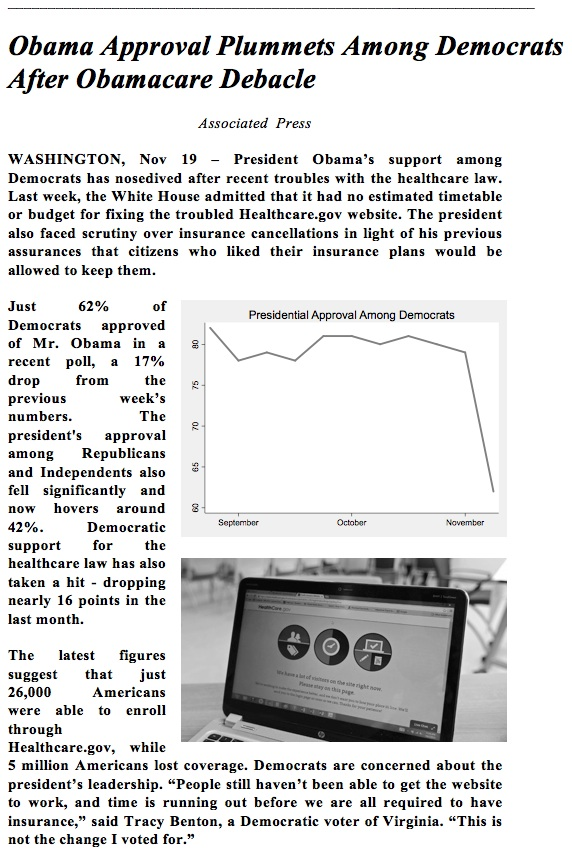
\includegraphics[width=1.05\textwidth]{../Manipulations/Dem_C.jpg}
\caption{Democrats Withdraw Support}
\label{fig:minipage1}
\end{minipage}
\quad
\begin{minipage}[b]{0.45\linewidth}
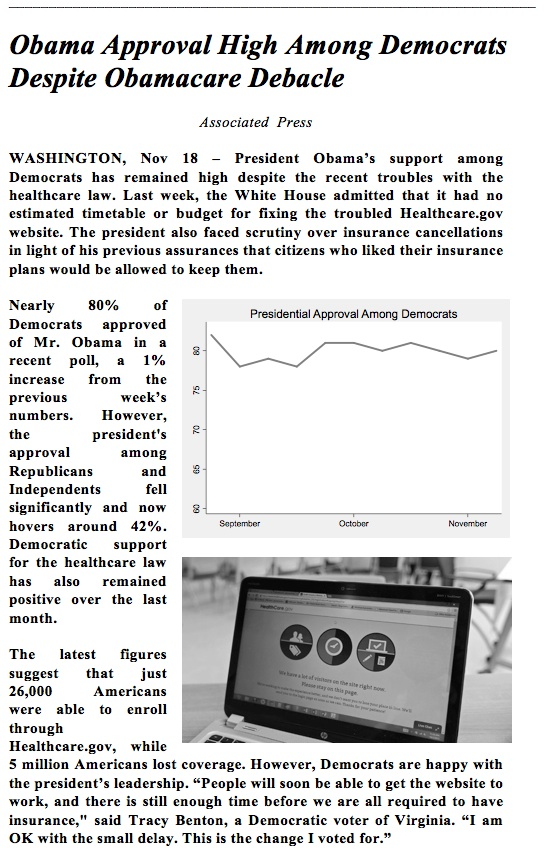
\includegraphics[width=1\textwidth]{../Manipulations/Dem_T.jpg}
\caption{Democrats Continue Support}
\label{fig:minipage2}
\end{minipage}
\end{figure}

\begin{figure}[ht]
\centering
\begin{minipage}[b][12cm][b]{0.45\linewidth}
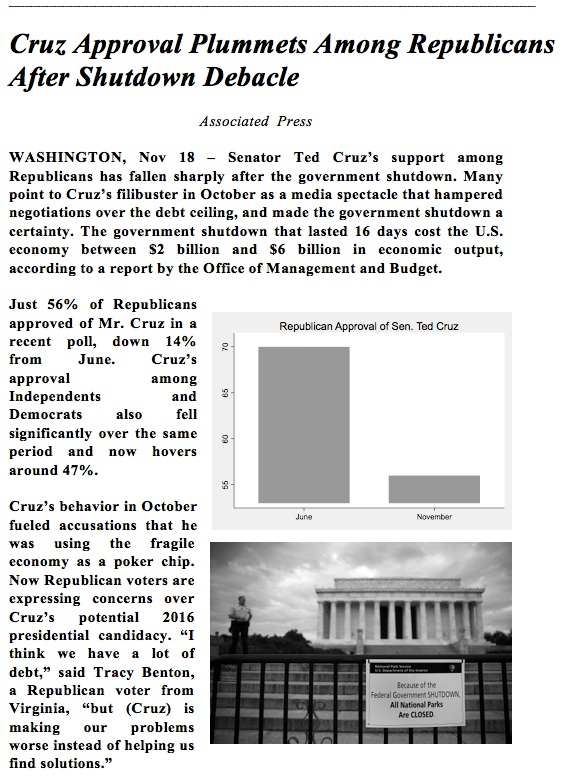
\includegraphics[width=1.05\textwidth]{../Manipulations/Rep_C.jpg}
\caption{Republicans Withdraw Support}
\label{fig:minipage3}
\end{minipage}
\quad
\begin{minipage}[b]{0.45\linewidth}
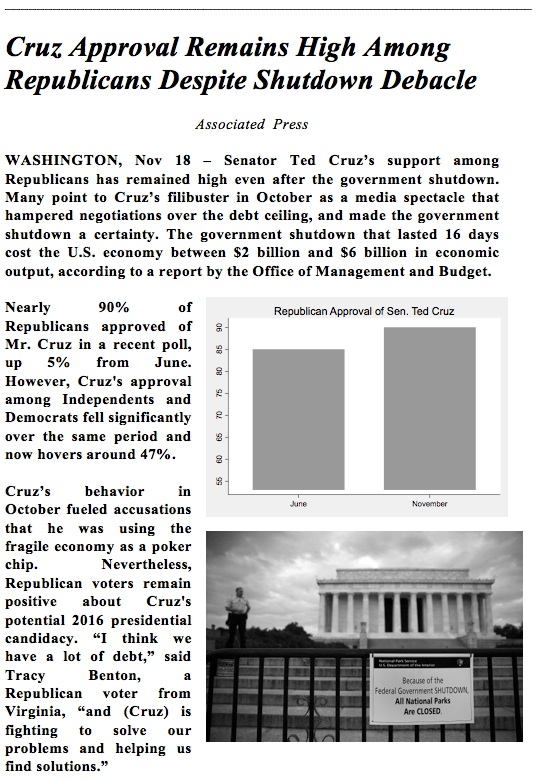
\includegraphics[width=1\textwidth]{../Manipulations/Rep_T.jpg}
\caption{Republicans Continue Support}
\label{fig:minipage4}
\end{minipage}
\end{figure}

\end{document}
